\section*{\fs{12}Zapytanie z użyciem Join}
\par{
\fs{12}

\subsection*{\fs{12} Raport z wyjazdu karetki w wybranym dniu.}
\listsinglespacing{
\fs{12}
\begin{lstlisting}[frame=single,language=SQL,]
Select * 
from Wyjazdy 
inner join Karetki on Karetki.id_karetki=Wyjazdy.id_karetki
Where Wyjazdy.data_wyjazdu='2022-02-25';

\end{lstlisting}
\begin{figure}[h!]
    \centering
   \scalebox{.85}{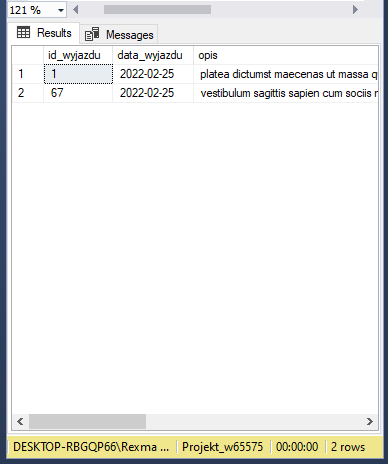
\includegraphics{Images/Zadanie3/P2/Z6a.png}}
    \caption{Wynik Zapytania}
    \label{fig:my_label}
\end{figure}

}
\begin{figure}[h!]
    \centering
   \scalebox{.60}{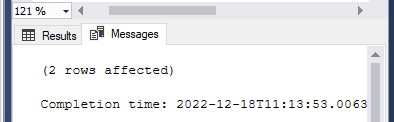
\includegraphics{Images/Zadanie3/P2/Z6b.png}}
    \caption{Wynik Zapytania}
    \label{fig:my_label}
\end{figure}
\newpage
\subsection*{\fs{12} Ilość zaplanowanych wizyt dla lekarza na dany dzień,}


\listsinglespacing{
\fs{12}
\begin{lstlisting}[frame=single,language=SQL,]
Select * 
from Wizyty inner join Pracownicy on Pracownicy.id_pracownika=Wizyty.lekarz
where Wizyty.data='2001-12-20';

\end{lstlisting}
\begin{figure}[h!]
    \centering
   \scalebox{.85}{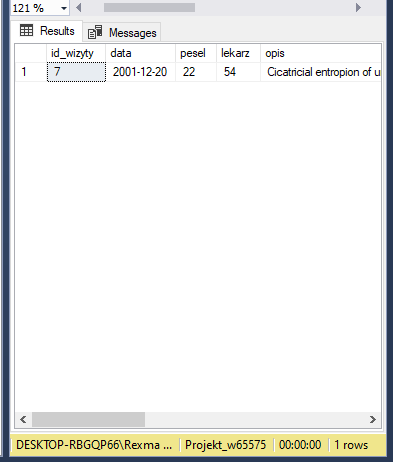
\includegraphics{Images/Zadanie3/P2/Z7a.png}}
    \caption{Wynik Zapytania}
    \label{fig:my_label}
\end{figure}

}
\begin{figure}[h!]
    \centering
   \scalebox{.60}{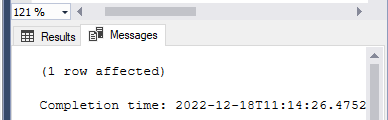
\includegraphics{Images/Zadanie3/P2/Z7b.png}}
    \caption{Wynik Zapytania}
    \label{fig:my_label}
\end{figure}
\newpage
\clearpage
\subsection*{\fs{12} Recepta dla Pacjenta }
\listsinglespacing{
\fs{12}
\begin{lstlisting}[frame=single,language=SQL,]
Create View Pacjent_Recepta as 
Select concat(P.imie,' ',P.nazwisko) as Pacjent , R.data,concat(PR.imie,' ',PR.nazwisko) as Lekarz,
LR.dawkowanie,L.nazwa,L.przeciwskazania,L.skład
from Pacjent as P
inner join Wizyty as W
on P.pesel=W.pesel 
inner join Recepta as R
on W.recepta=R.id_recepty
inner join Pracownicy as PR
on PR.id_pracownika=R.lekarz
inner join lekarstwa_recepty as LR
on LR.id_recepty=R.id_recepty
inner join Lekarstwa as L
on L.id_lekarstwa=LR.id_lekarstwa

Select * from [Pacjent_Recepta]
where YEAR(data) between 2000 and 2010

\end{lstlisting}
\begin{figure}[h!]
    \centering
   \scalebox{.85}{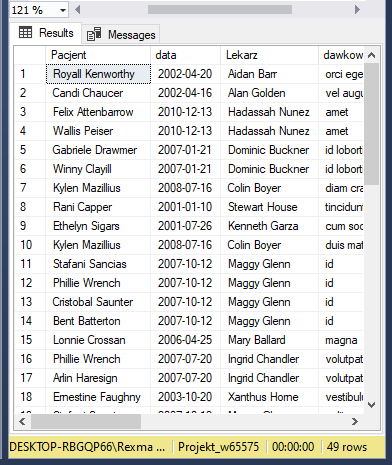
\includegraphics{Images/Zadanie3/P2/Z8a.png}}
    \caption{Wynik Zapytania}
    \label{fig:my_label}
\end{figure}

}

\begin{figure}[h!]
    \centering
   \scalebox{.70}{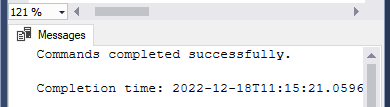
\includegraphics{Images/Zadanie3/P2/Z8b.png}}
    \caption{Wynik Zapytania}
    \label{fig:my_label}
\end{figure}
\newpage
\clearpage
\subsection*{\fs{12} Numery,Opisy wyjazdów i leki użyte podczas interwencji }
\listsinglespacing{
\fs{12}
\begin{lstlisting}[frame=single,language=SQL,]

Select W.id_wyjazdu,W.data_wyjazdu, W.opis, L.nazwa
from Lekarstwa as L
inner join lekarstwa_wyjazdy as LW
on LW.id_lekarstwa=L.id_lekarstwa
inner join Wyjazdy as W
on W.id_wyjazdu=LW.id_wyjazdu


\end{lstlisting}
\begin{figure}[h!]
    \centering
   \scalebox{.85}{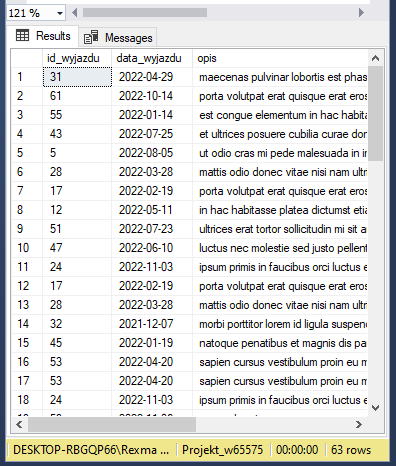
\includegraphics{Images/Zadanie3/P2/Z9a.png}}
    \caption{Wynik Zapytania}
    \label{fig:my_label}
\end{figure}

}

\begin{figure}[h!]
    \centering
   \scalebox{.70}{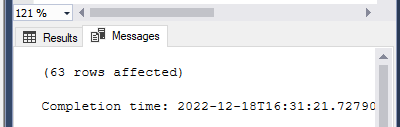
\includegraphics{Images/Zadanie3/P2/Z9b.png}}
    \caption{Wynik Zapytania}
    \label{fig:my_label}
\end{figure}
\newpage
\clearpage

\subsection*{\fs{12} Badania których wyniki są powyżej normy      }
\listsinglespacing{
\fs{12}
\begin{lstlisting}[frame=single,language=SQL,]
Select Nazwa, Wyniki.wynik,Wyniki.normy
from Badania
inner join Wyniki
on Wyniki.id_wynikow=Badania.wyniki
where wynik>normy

\end{lstlisting}
\begin{figure}[h!]
    \centering
   \scalebox{.85}{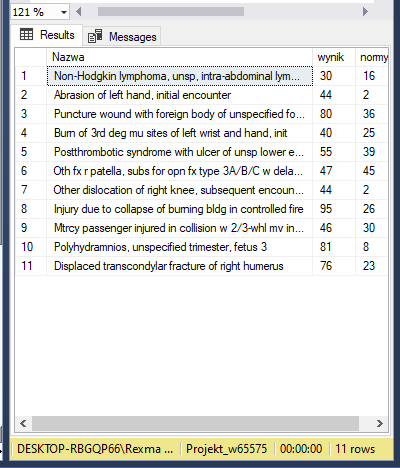
\includegraphics{Images/Zadanie3/P2/Z10a.png}}
    \caption{Wynik Zapytania}
    \label{fig:my_label}
\end{figure}

}

\begin{figure}[h!]
    \centering
   \scalebox{.70}{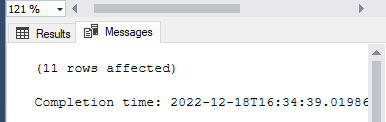
\includegraphics{Images/Zadanie3/P2/Z10b.png}}
    \caption{Wynik Zapytania}
    \label{fig:my_label}
\end{figure}
\newpage
\clearpage